\documentclass{report}

\usepackage{apalike}
\usepackage{graphicx}
\usepackage{url}
\bibliographystyle{apalike} 

\title{replace title}
\author{replace author}
\date{replace date}

\begin{document}
\maketitle
\tableofcontents
\listoffigures

\chapter{Introduction}

\chapter{Executive Summary}
\section{Planning}
\subsection{Approach}
\subsection{Scope}
\subsection{Objectives}
\section{Methodology}
\subsection{Information Gathering}
\subsection{System Attacks}
\section{Summary of Findings}

\chapter{Key Findings}


\section{Auction Site}
This section covers the vulnerabilities found with the user-facing auction site.
\subsection{Path Traversal}
\subsubsection{Security Implications / Risk Level}
Path traversal allows for arbitrary file read across the system, for any files readable by the apache user (www-data). This is dangerous as it could potentially leak sensitive company data, as well as user data. If combined with other vulnerabilities, such as incorrect permissions on log files, it is possible to achieve Remote Code Execution through malicious log read/write.\\
Overall, the execution of this vulnerability is trivial, and the repercussions are potentially serious but not disastrous. Due to this, the risk level of this vulnerability is evaluated to be \textbf{medium}.
\subsubsection{Cause of Vulnerability}
The vulnerability is caused by the method used to retrieve and display image files on the website. Instead of directly referencing the image file through the 'src' field on an 'img' HTML tag, a PHP script is instead used to include the file.\\ 
While using PHP include scripts may not normally be dangerous, the file name to be retrieved can be edited by the user, allowing them to easily select which file should be displayed. A lack of filter/extension whitelist makes this even more potent.
\subsubsection{Steps to Replicate}
\begin{itemize}
		\item Firstly the inspect element tool in Mozilla Firefox was used to inspect an image, revealing the image URL (Fig. 3.1).
		\item The image URL could then be opened, showing the ASCII representation of the binary content for the image file (Fig. 3.2).
		\item Finally, the URL parameter 'file' could be replaced with a file path, allowing for arbitrary file read. In this example, the ../ operator was used to go up directories until root, and then the /etc/passwd file was navigated to (Fig. 3.3).
\end{itemize}
\begin{figure}[!htb]
	\centering
	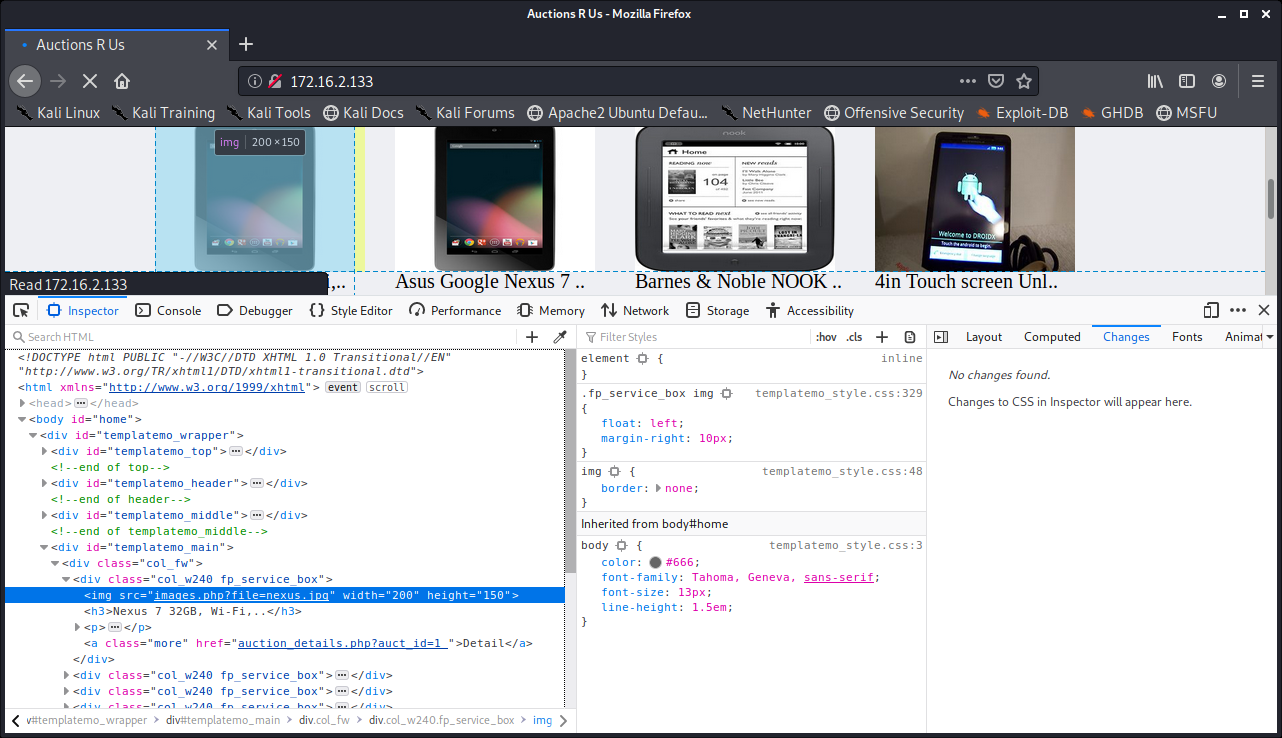
\includegraphics[scale=0.4]{img/pathtraversal1.png}
	\caption{Inspecting the image}
\end{figure}
\begin{figure}[!htb]
	\centering
	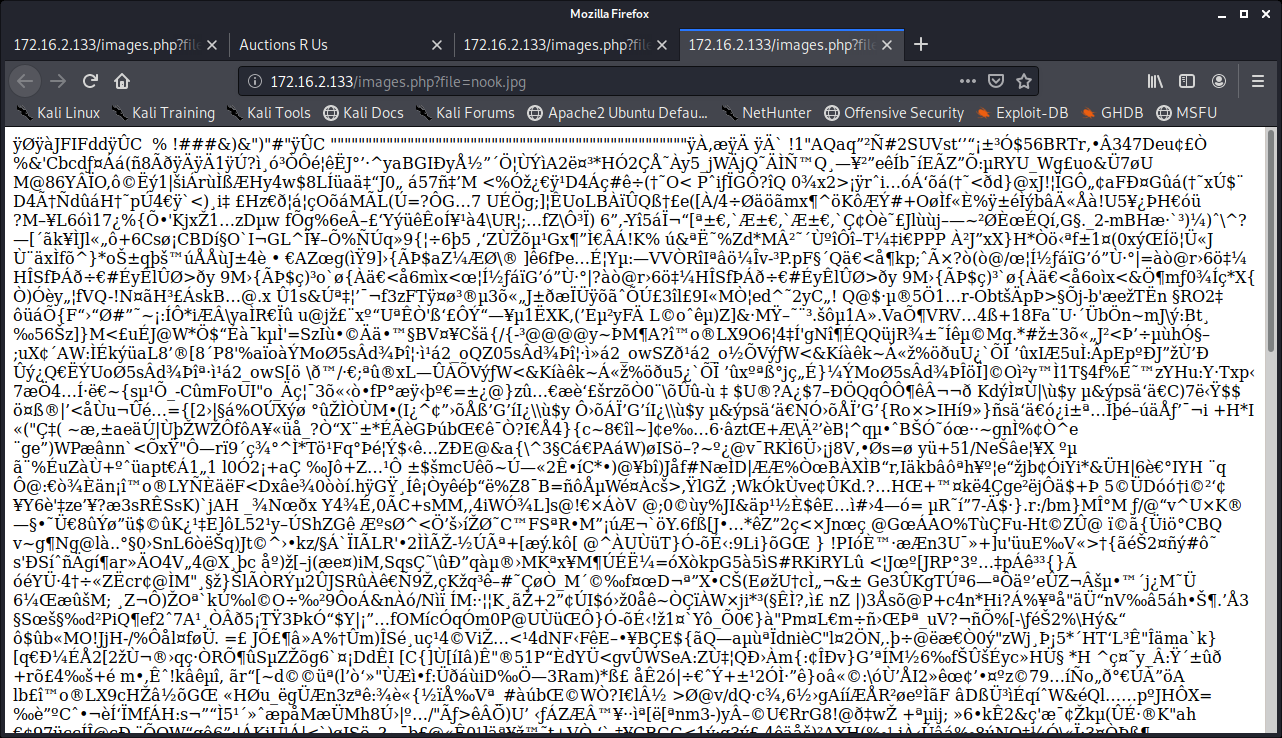
\includegraphics[scale=0.4]{img/pathtraversal2.png}
	\caption{Viewing the image contents}
\end{figure}
\begin{figure}[!htb]
	\centering
	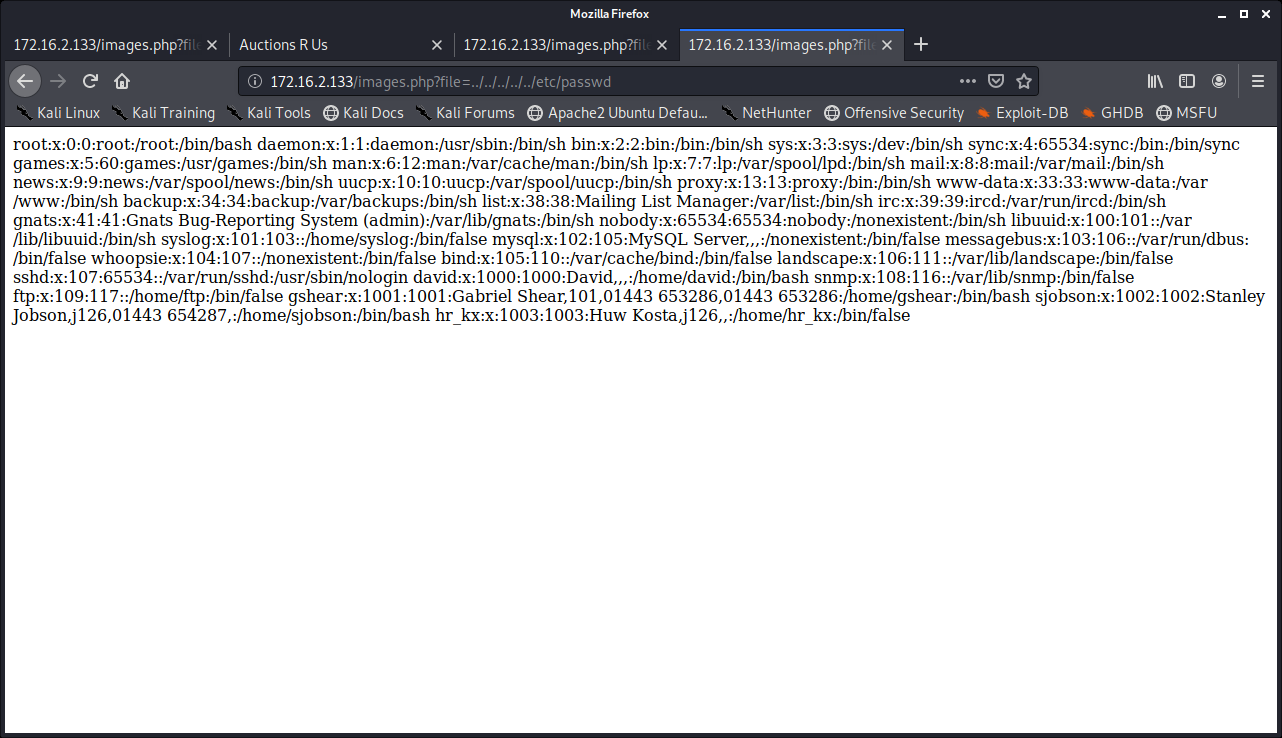
\includegraphics[scale=0.4]{img/pathtraversal3.png}
	\caption{Exploiting the vulnerable file read}
\end{figure}
\pagebreak



\subsection{SQL Injection}
\subsubsection{Security Implications / Risk Level}
SQL injection is a blanket term covering any kind of unintended user control over the SQL queries interacting with a database. This can manifest in many forms, such as:
\begin{itemize}
	\item Authentication bypass, where SQL queries can be modified to bypass authentication checks such as login forms.
	\item Union injection, where the UNION keyword in SQL can be used to access data from other columns, tables, and databases.
	\item Error based injection, where SQL errors are intentionally created in order to gain information about the database.
	\item Blind injection, where queries that return TRUE or FALSE can be used to gain information about the database.
\end{itemize}
From the testing done, the website appears to be vulnerable to both authentication bypass, allowing attackers to log in to accounts, and blind injection, allowing for full read access across the database.\\
The execution of these vulnerabilities are relatively easy with the use of tools like SQLmap, and the repercussions can be very serious, allowing attackers to log in to administrator accounts as well as reading any user/auction data from the database. Due to this, the risk level of this vulnerability is evaluated to be \textbf{high}.
\subsubsection{Cause of Vulnerability}
SQL injection vulnerabilities are a result of allowing unsanitised user input in to SQL queries. Sanitising SQL queries involves removing any kind of dangerous character from the input, such as quotation marks (single and double) and comment tags. If this is not done, attackers are able to modify queries in specific ways to allow them to perform SQL injection.\\
One example of this would be performing an authentication bypass injection. A normal query may use a query like:
\begin{verbatim}
SELECT * FROM users WHERE username = '$inputname' AND password = 
'$inputpass';
\end{verbatim}
If an attacker enters something like ' OR 1=1\# in to the username field, the query becomes:
\begin{verbatim}
SELECT * FROM users WHERE username = '' OR 1=1#;
\end{verbatim}
Which will pick the first username from the table and sign the attacker in.
\subsubsection{Steps to Replicate}
\begin{itemize}
	\item For initial testing of SQL injection, a basic authentication bypass was used. The payload ' OR 1=1-- - was entered in to the username field (Fig. 3.4), which subsequently allowed access to the 'David' account, giving use of the admin panel as well (Fig. 3.5).
	\item For further testing, the tool SQLmap was used. This is a tool that automatically iterates through potential SQLi payloads, providing information such as DB names, table names, table data, SQL user names, and SQL version.
	\item The first test done with SQLmap was checking if it detected SQL injection. The command used for this was \begin{verbatim}sqlmap -u "http://172.16.2.133/login.php?username=qwe&
	password=qwe&Search=" --batch\end{verbatim}The results provided some information on the DB system and potential attacks it was vulnerable to (Fig. 3.6).
	\item After this, the --passwords flag was used to test for DB users and retrieve any passwords if possible. SQLmap found a DB user named "auctuser", but had no access to the users table so could not retrieve a password (Fig. 3.7).
	\item With no password found, the next step was to search for databases. The command used to do this was
\begin{verbatim}
sqlmap -u "http://172.16.2.133/login.php?username=qwe&
password=qwe&Search=" --batch --databases
\end{verbatim}
	This successfully found the databases, returning three in total (Fig. 3.8). The first was the information\_schema DB, default in all installations of MySQL. The second was the auctionsrus DB, the one likely holding all info. The last was a test DB which also comes default with MySQL.
	\item With the new information of the auctionsrs db, the --tables flag could be used to dump the table names for said DB. The command used for this was:
\begin{verbatim}
sqlmap -u "http://172.16.2.133/login.php?username=qwe&
password=qwe&Search=" --batch -D auctionsrus --tables
\end{verbatim}
	This returned two tables found in the auctionsrus DB (Fig. 3.9). One, auction\_users, was likely to contain the user data for the site, while the other, auctions, was likely to contain the auction data.
	\item Finally, the last step was to attempt to dump the data from the tables. As a proof of concept, the data from the users table was dumped using the command:
\begin{verbatim}
sqlmap -u "http://172.16.2.133/login.php?username=qwe&
password=qwe&Search=" --batch -D auctionsrus -T auction_users --dump
\end{verbatim}
	This returned the full set of user data from the auction\_users table, including usernames, MD5 hashed passwords (all cracked, with the one not displayed on the screenshot being '7331'), user IDs, and user levels (Fig. 3.10). With the dump done, the full extent of the SQL injection was explored.
\end{itemize}
\pagebreak
\begin{figure}[!htb]
	\centering
	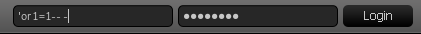
\includegraphics[scale=1]{img/sqli1.png}
	\caption{Authentication bypass SQLi}
\end{figure}
\begin{figure}[!htb]
	\centering
	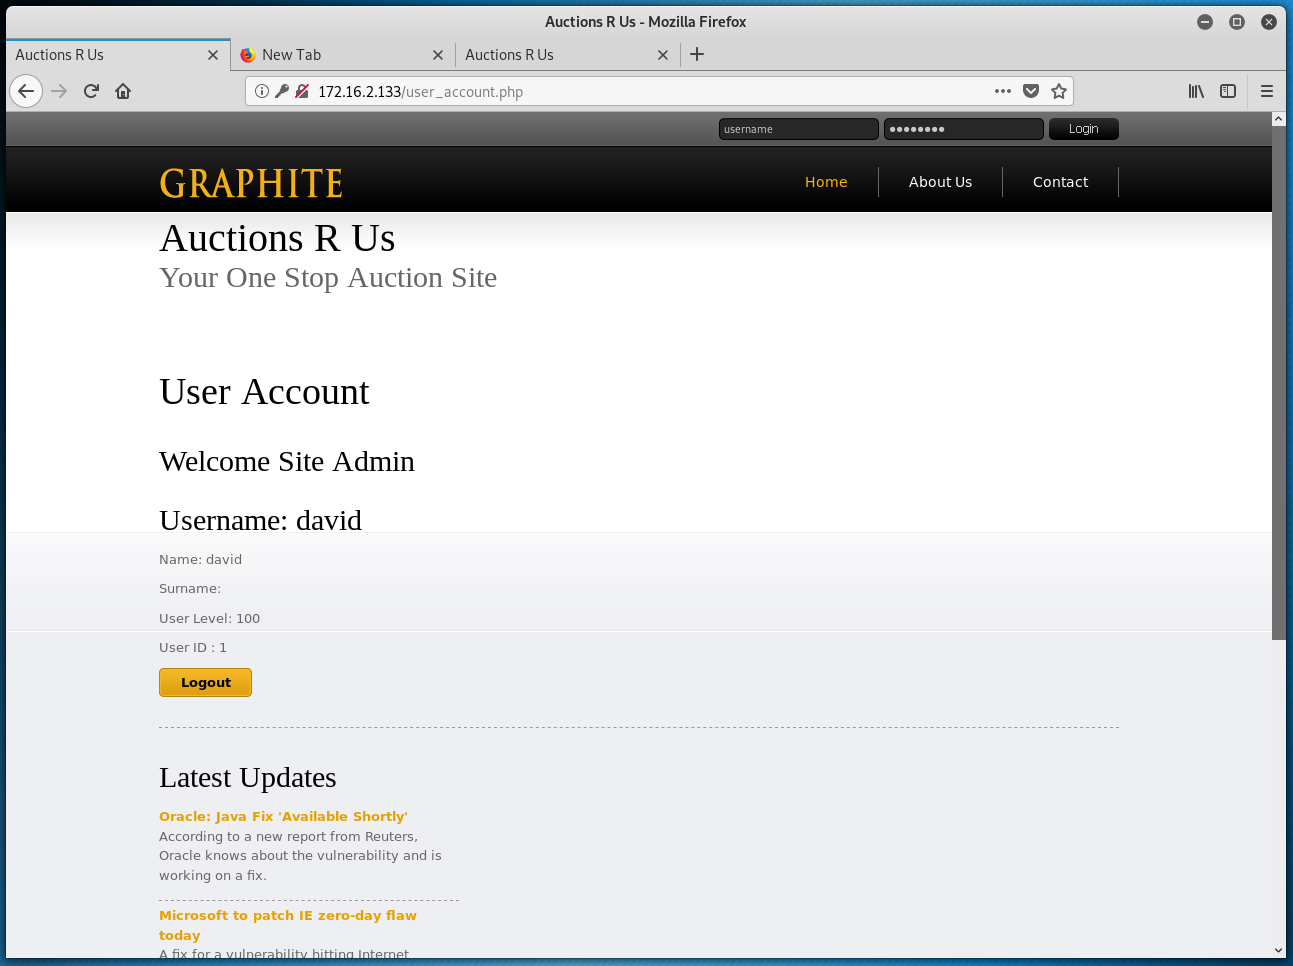
\includegraphics[scale=0.4]{img/sqli2.png}
	\caption{Admin panel access gained}
\end{figure}
\begin{figure}[!htb]
	\centering
	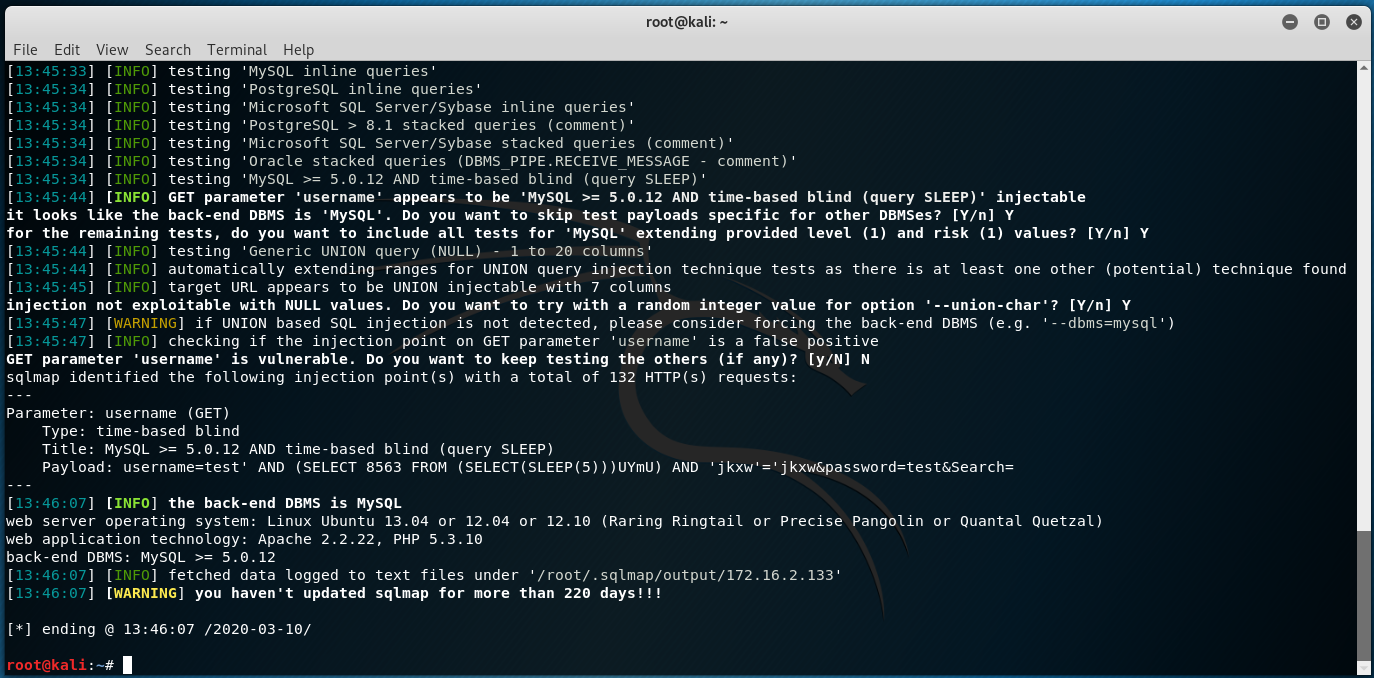
\includegraphics[scale=0.3]{img/sqlmap1.png}
	\caption{Initial SQLmap testing}
\end{figure}	
\begin{figure}[!htb]
	\centering
	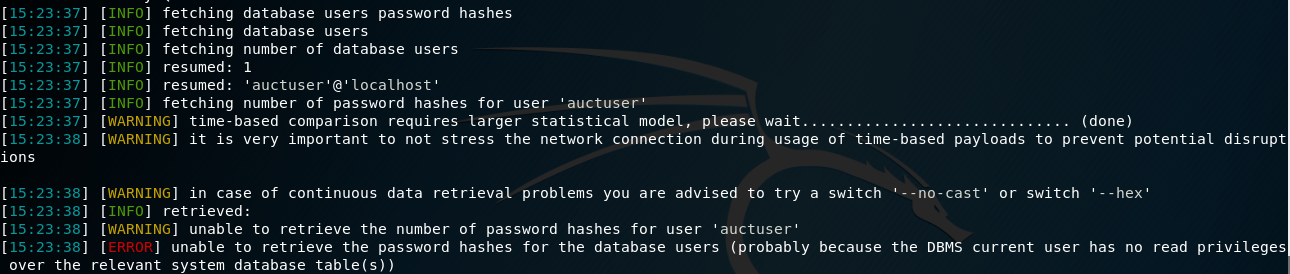
\includegraphics[scale=0.4]{img/sqlmap1.5.png}
	\caption{Finding DB users}
\end{figure}
\begin{figure}[!htb]
	\centering
	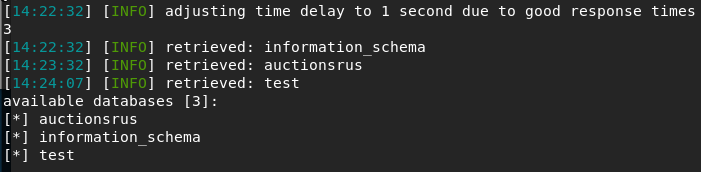
\includegraphics[scale=0.6]{img/sqlmap2.png}
	\caption{Finding DB names}
\end{figure}
\begin{figure}[!htb]
	\centering
	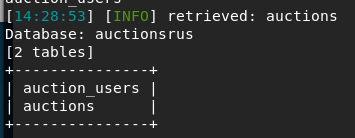
\includegraphics[scale=0.7]{img/sqlmap3.png}
	\caption{Finding table names}
\end{figure}
\begin{figure}[!htb]
	\centering
	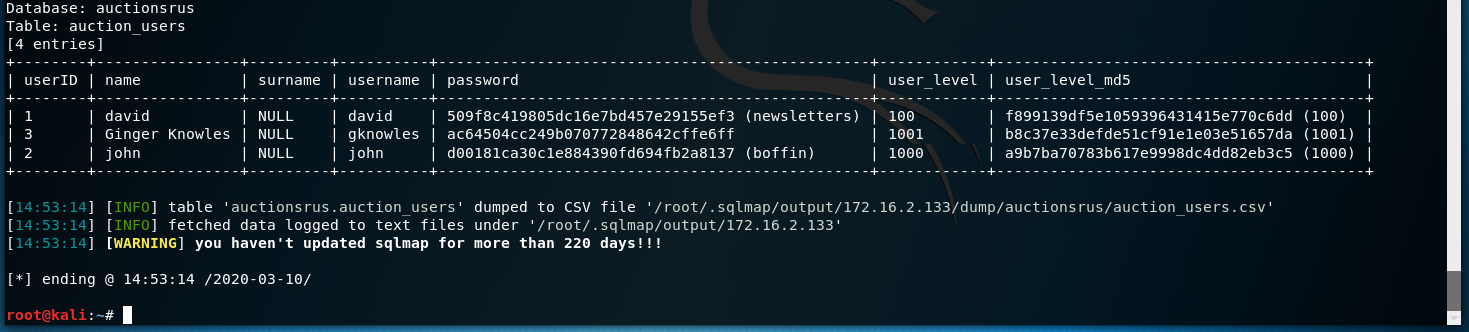
\includegraphics[scale=0.3]{img/sqlmap4.png}
	\caption{Dumping user data}
\end{figure}
\pagebreak

\subsection{Weak Authentication}
\subsubsection{Security Implications / Risk Level}
Weak authentication is another blanket term for a multitude of security vulnerabilities surrounding the authentication systems on a website. Again, these vulnerabilities can manifest in a number of forms, and have varying levels of risk depending on the vulnerability.\\
During testing a number of vulnerabilities were found that could be classed under weak authentication. These were:
\begin{itemize}
	\item Susceptibility to bruteforce attacks: There appeared to be no rate-limiting or IP blocking functionality on the website login form, allowing for bruteforce attacks to be performed easily. These attacks could potentially result in user accounts being accessed by attackers.
	\item Weakly hashed passwords: Using SQLmap, the users table was dumped, revealing that the passwords were hashed with unsalted MD5. This is a very weak algorithm, allowing it to be cracked quickly, as well as it having a plethora of rainbow tables already available online. This could result in threat actors easily cracking passwords if they were able to retrieve the hashes.
	\item Weak session IDs: Instead of a secure session ID, the session IDs used within the website are simply an MD5 hash of the user level for that account. This is extremely dangerous, as an attacker can easily enumerate through the user levels, testing each one and gaining access to every account with ease.
Due to the numerous vulnerabilities possible with weak authentication, and the dangerous ability to get in to other accounts (including admins), this vulnerability is evaluated to be a \textbf{high} risk.
\end{itemize}

\subsubsection{Cause of Vulnerability}
The vulnerabilities found each had varying causes, depending on which part of the website was being interacted with. These included:
\begin{itemize}
	\item Susceptibility to bruteforce attacks: The lack of a rate-limit or IP block on each account for the login form allows attackers to attempt as many times as they want, which makes bruteforce attacks possible. 
	\item Weakly hashed passwords: The use of the MD5 hashing algorithm results in weak hashing security, which stems from either legacy code (from when MD5 was stronger) or poor security choices during the design of the system.
	\item Weak session IDs: Again, this is another issue stemming from poor security choices during the design stage. Session IDs should be chosen as a completely random string, so threat actors cannot collate multiple hashes and find patterns between them. Using unsalted MD5 as the hashing algorithm for this makes it even worse, as it is very easy to reverse engineer the original text from the hashes due to the nature of the user ID being numeric.
\end{itemize}

\subsubsection{Steps to Replicate}
Bruteforcing the login form
\begin{itemize}
	\item To bruteforce the login form, a custom python script was used (Appendix A). This script read in usernames from a 'usernames.txt' file, and passwords from a provided wordlist (in this case english top 10000 wordlist). For each username, the script iterated through the passwords, sending a GET request using the python 'requests' library. If the text 'User Account' was found in the response text, this would indicate a successful sign in and print the found credentials before moving on to the next username.
	Using the script successfully found the credentials for the admin user 'david' (Fig. 3.11), and could likely find the rest if a more extensive wordlist was used.	
\end{itemize}
Cracking the password hashes from SQLmap
\begin{itemize}
	\item The password hashes gained from SQLmap were unsalted MD5, so one of the first things to check would be an online rainbow table (a database of hashes and their corresponding plaintexts). In this case, the website 'Crackstation' was used to reverse all three hashes (Fig. 3.12).
\end{itemize}
Enumerating the session IDs
\begin{itemize}
	\item To enumerate the session IDs, another custom python script was created (Appendix B). This script enumerated through the numbers 0-1500, hashing each number of iteration. With the hash, the requests library was again used to send a GET request to the user\_account.php page, with the hash set as a cookie. The response text of the request could then be analysed - first to check if any sign in was detected, which would then print the hash used, user level, and username. It would then check if the admin panel text was present, and if so, print that the user was an admin. This method was used to gain access to all 3 auction accounts (Fig. 3.13).
\end{itemize}
\begin{figure}[!htb]
	\centering
	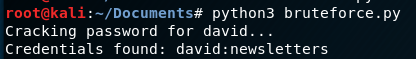
\includegraphics[scale=0.7]{img/bruteforce1.png}
	\caption{Bruteforcing the David user}
\end{figure}
\begin{figure}[!htb]
	\centering
	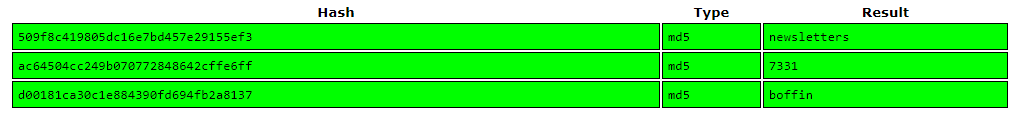
\includegraphics[scale=0.5]{img/crackstation.png}
	\caption{Cracking the hashes from SQLmap}
\end{figure}
\begin{figure}[!htb]
	\centering
	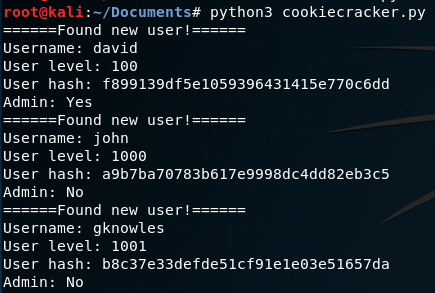
\includegraphics[scale=0.6]{img/cookie1.png}
	\caption{Enumerating the session IDs}
\end{figure}



\section{SRV1 - Windows Server}
\subsection{RDP Bruteforce}
\subsubsection{Security Implications / Risk Level}
RDP, or Remote Desktop Protocol, is a service used for remotely accessing machines across a network. While it is a useful tool for remote administration, it can be very heavily exploited by an attacker if not properly secured, as it gives almost full access to the machine if compromised. \\
In this situation, the system was vulnerable to an RDP bruteforce. Using this vulnerability, it was possible to gain access to the 'ftp' user, creating a foothold in to the system which could be further exploited.\\
Due to the risk of accessing accounts on the server machine, but still requiring passwords which could potentially mitigate the potential of exploitation, this vulnerability is classed at \textbf{medium} risk.
\subsubsection{Cause of Vulnerability}
This vulnerability stemmed from the RDP port (3389) being left open on the server. Having the default RDP port open allows threat actors to easily identify the service running on the port, giving away a potential entry point to the system. From there, any bruteforce program such as hydra or ncrack can be used to begin bruteforce attempts on the service.
\subsubsection{Steps to Replicate}
\begin{itemize}
	\item First, a list of potential usernames was collated from information gathered previously - this included usernames of known staff members (such as Stanley Jobson and Gabriel Shear), as well as common account names (such as guest and ftp). 
	\item Next, the tool Hydra was used along with the rockyou.txt wordlist to start an RDP bruteforce, using the command 
	\begin{verbatim}
		hydra -t 4 -l ftp -P rockyou.txt rdp://172.16.2.135 -v
	\end{verbatim}
	This command allocates 4 tasks to the bruteforce, uses the username 'ftp' (each username was inputted manually), the password list as rockyou.txt, and the target as 172.16.2.135, the IP of the server.
	\item After trying multiple other user accounts without success, the bruteforce eventually returned a set of credentials for the 'ftp' user - 'ftp:Abracadabra' (Fig. 3.14). These credentials were then used with the Linux utility 'rdesktop' to remote in to the machine, successfully gaining access to the server (Fig. 3.15).
\end{itemize}
\begin{figure}[!htb]
	\centering
	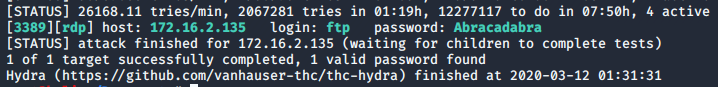
\includegraphics[scale=0.6]{img/rdp1.png}
	\caption{Bruteforcing the ftp user credentials}
\end{figure}
\begin{figure}[!htb]
	\centering
	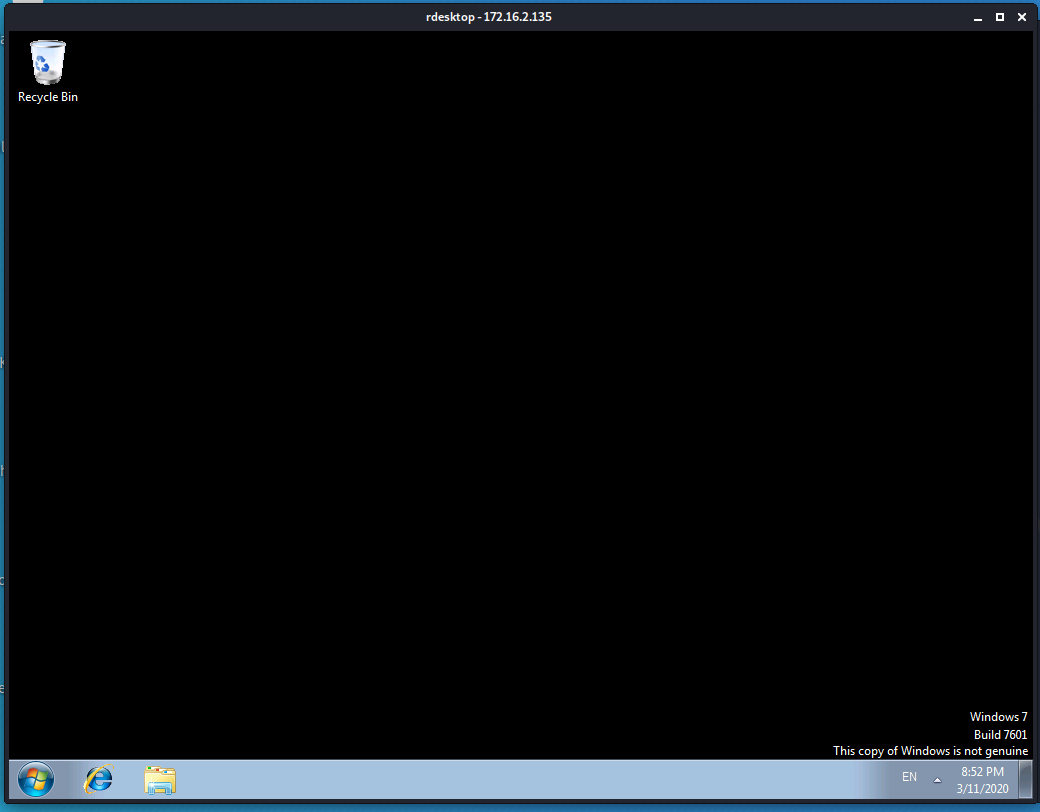
\includegraphics[scale=0.4]{img/rdp2.png}
	\caption{Gaining access to the server through RDP}
\end{figure}
\pagebreak

\subsection{Insecure Privileges}
\subsubsection{Security Implications / Risk Level}
Insecure privilege attacks occur when system privileges are distributed in a way that allows for attackers to exploit them moreso than if the privileges were configured correctly. Some examples of this include giving every user administrator privileges on a Windows machine, or making all files global R/W/X on a Linux machine. Doing this allows the attacker to exploit the machines much more heavily than if users had their permissions restricted, or if files were correctly configured.\\
In this situation, the ftp user was given administrator privileges, which allowed for escalation to the system user as well as dumping the NT password hashes for every user on the machine. This is a huge security flaw, as if the ftp account was breached (as it was using the RDP bruteforce), the attacker gains full administrator privileges on the target machine. Due to this, the risk level was evaluated to be \textbf{high}.
\subsubsection{Cause of Vulnerability}
The cause of this vulnerability would come down to lack of security considerations when administering permissions to system users. As the ftp user should only be used for file transfers, there is no reason it should have administrative privileges.
\subsubsection{Steps to Replicate}
\begin{itemize}
	\item After logging in to the ftp user with rdesktop using the credentials from the RDP bruteforce, the user's privileges were checked with the 'net user ftp' command (Fig. 3.16).
	\item From here, the next step was to use the PsExec tool to escalate to the system user. The PsTool suite is not installed by default, and with no internet connection, another method had to be used to transfer the files across. The method used in this case was by creating a linked RDP share with rdesktop, using the command
	\begin{verbatim}
		rdesktop 172.16.2.135 -r disk:share=/root/Documents/pentest
	\end{verbatim}
This linked the /root/Documents/pentest folder on the host machine to the 'share' folder on the network drive. From here, the PsExec files could be transferred from the host to the server (Fig. 3.17).
	\item With PsExec now on the server, it could be used to elevate to system user by using the command
	\begin{verbatim}
	PsExec.exe -i -s cmd.exe
	\end{verbatim}
	With this entered, a new shell is spawned running as nt authority/system, giving full privileges over the server (Fig. 3.18).
\end{itemize}

\begin{figure}[!htb]
	\centering
	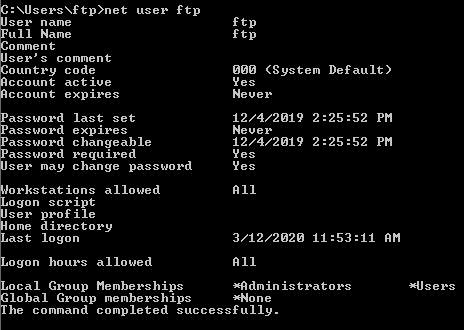
\includegraphics[scale=0.6]{img/privesc1.png}
	\caption{Checking user permissions for ftp}
\end{figure}
\begin{figure}[!htb]
	\centering
	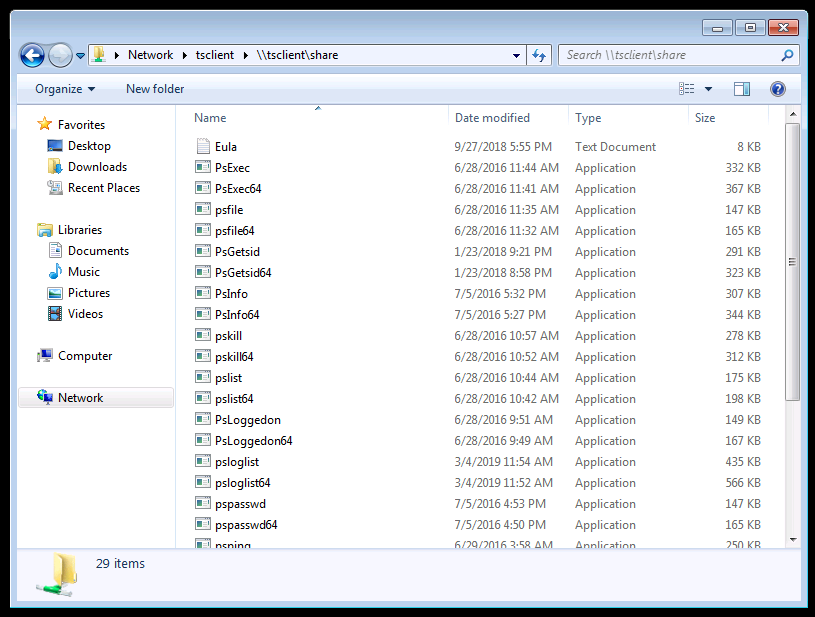
\includegraphics[scale=0.5]{img/privesc2.png}
	\caption{Using a file share to transfer PsExec}
\end{figure}
\begin{figure}[!htb]
	\centering
	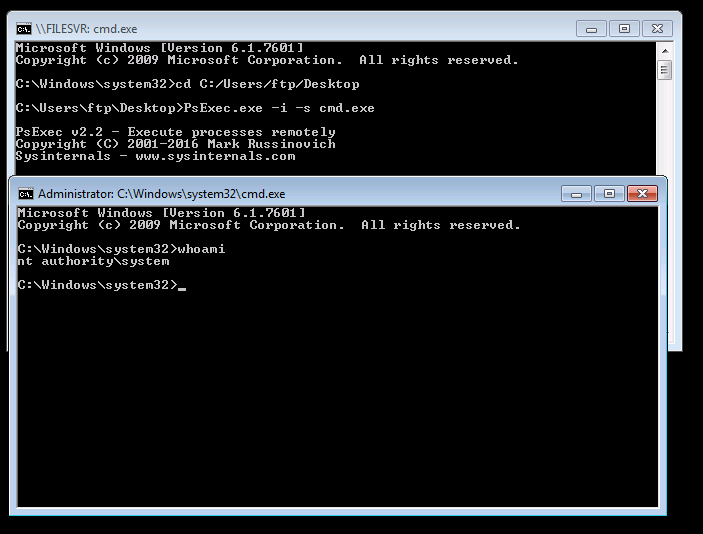
\includegraphics[scale=0.5]{img/privesc3.png}
	\caption{Elevating to system}
\end{figure}
\pagebreak

\subsection{Weak passwords}
\subsubsection{Security Implications / Risk Level}
Weak passwords involve passwords that do not stand up to modern hash cracking techniques. This can be caused by a number of factors, such as
\begin{itemize}
	\item Not having a long enough password - even passwords with up to 8 characters can be cracked feasibly within days \cite{passwordcracking}
	\item Not using symbols and numbers - using symbols and numbers exponentially increases the keyspace required to crack the password. Not doing so will make it much easier for threat actors to potentially crack the plaintext.
	\item Using common passwords - threat actors often use wordlists instead of plain bruteforce nowadays, with wordlists containing millions of common passwords available online such as rockyou. There are many ways to check if a password has already been leaked, such as the online tool HaveIBeenPwned, which collates password lists and allows users to check if a password appears in them.
\end{itemize}
These passwords would be crackable when using a weak hash type (such as NT) on a local machine, but doing so on a remote machine would not be as feasible. Therefore, the risk level is evaluated as \textbf{low}.
\subsubsection{Cause of Vulnerability}
The cause of this vulnerability is simply not choosing a password that is sure enough. Individual users are often blamed for creating weak passwords, but in practise the responsibility is on the administrators to set a strong password policy in order to force users to use a secure password. Doing this will ensure user passwords are much less likely to be cracked, preventing easy entry in to internal systems.
\subsubsection{Steps to Replicate}
\begin{itemize}
	\item The first step was to extract the password hashes from the server. As system access was gained with PsExec, it was possible to use Pwdump7 to extract the hashes from the SAM directory in Windows. The Pwdump7 executable was transferred across using the same RDP file share used for PsExec, and then ran on the system to get the hashes (Fig. 3.19).
	\item This produced seven hashes, one for each user on the machine. These hashes were then transferred to a text file on a host Windows 10 machine to prepare for cracking.
	\item To crack the hashes, the tool 'hashcat' was used. This tool is especially suited for the job as it is GPU accelerated, meaning if a powerful GPU is available, it is possible to crack many more hashes than a CPU-bound program such as John the Ripper.
	\item The first crack done with hashcat was using the 'rockyou.txt' wordlist, without any additional rules. Doing this yielded two passwords, 'ftp:Abracadabra' which was already gained through RDP bruteforce, and 'James Reisman:xylophone', which was a standard user account (Fig. 3.20).
	\item The next crack was done using rockyou again, but with the 'best64' ruleset. A ruleset is a feature available in hashcat to mutate passwords from a wordlist, changing them in predictable ways - for example, the 'leetspeak' ruleset would go through each word in the list applying leetspeak to it (hello > h3ll0). The best64 ruleset utilises some of the most effective hashcat rules, while still running in a relatively short time. Using this, another hash was cracked - 'Administrator:zarpazos' (Fig. 3.21).
	\item The next crack was similar to the last, but using the 'd3ad0ne' ruleset instead of best64. This ruleset is significantly larger, which trades off increased time to crack with more potential password candidates to go through. This ruleset produced a great result, giving another 2 cracked hashes - 'Holly Jobson:try2catchMe' and 'Ginger Knowles:G1ng3rK' (Fig. 3.22).
	\item The final crack performed was with a 'hybrid attack'. This is done by taking a dictionary (rockyou.txt), and a 'mask' (a feature used in hashcat for expressing specific character sets). These two are then combined, resulting in a combination of a wordlist and a bruteforce. For this, the mask type ?a was used, which contains all lowercase, uppercase, numerical, and symbol characters.\\ 
	The hybrid attack was repeated with varying lengths of bruteforce - as each bruteforce needs to be applied to every character in the wordlist, it can quickly become too large to compute. In this case, doing it with lengths up to 3 were completable in reasonable time.\\
	This attack yielded one hash when executed with rockyou as the dictionary and ?a?a?a as the mask - 'Gabriel Shear:donttrustN31' (Fig. 3.23). This was the last hash that was cracked.
	\item In total, six hashes were able to be cracked (Fig. 3.24). The seventh (Stanley Jobson's) seems stronger, and would require more testing to see if it is crackable.
\end{itemize}

\begin{figure}[!htb]
	\centering
	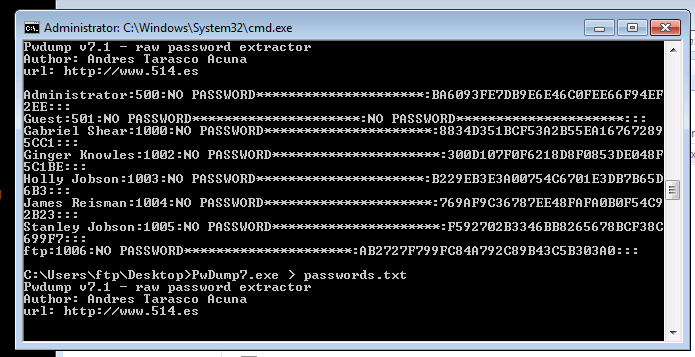
\includegraphics[scale=0.7]{img/hashdump1.png}
	\caption{Using Pwdump7 to extract hashes}
\end{figure}
\begin{figure}[!htb]
	\centering
	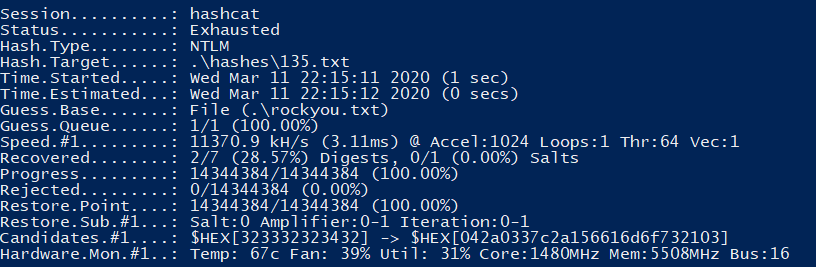
\includegraphics[scale=0.5]{img/hashdump2.png}
	\caption{Cracking two hashes with standard rockyou}
\end{figure}
\begin{figure}[!htb]
	\centering
	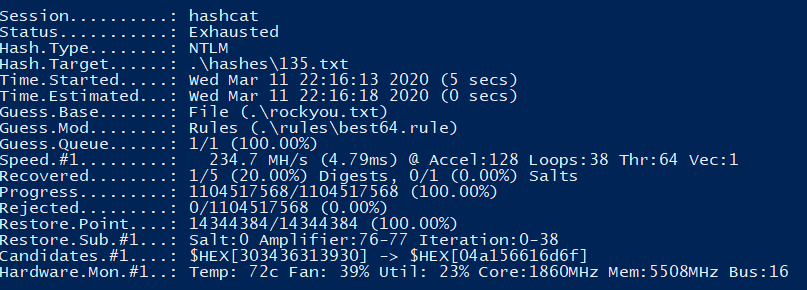
\includegraphics[scale=0.6]{img/hashdump3.png}
	\caption{Cracking one hash with rockyou + best64}
\end{figure}
\begin{figure}[!htb]
	\centering
	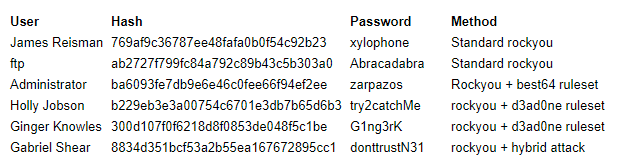
\includegraphics[scale=0.6]{img/hashdump4.png}
	\caption{Cracking two hashes with rockyou + d3ad0ne}
\end{figure}
\begin{figure}[!htb]
	\centering
	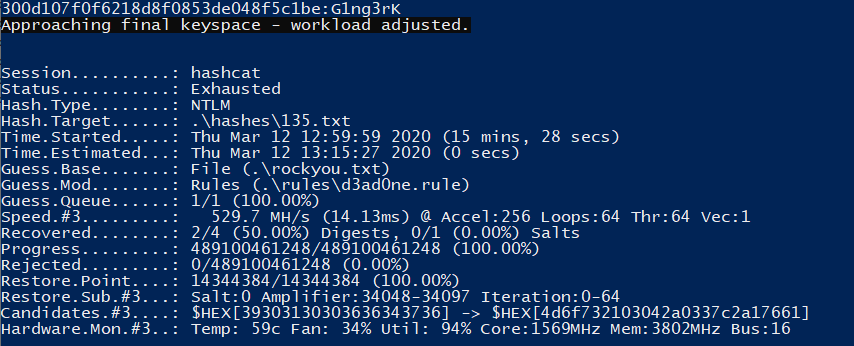
\includegraphics[scale=0.6]{img/hashdump5.png}
	\caption{Cracking one hash with rockyou hybrid attack}
\end{figure}
\begin{figure}[!htb]
	\centering
	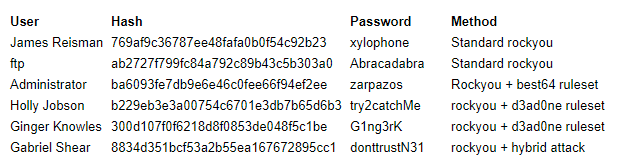
\includegraphics[scale=0.6]{img/hashdump6.png}
	\caption{Final results of hash cracking}
\end{figure}
\pagebreak



\section{Ubuntu Client}
\subsection{FTP Anonymous Access}
\subsubsection{Security Implications / Risk Level}
By default, FTP allows for access without password authentication through the 'anonymous' user. While this user does not have many permissions, it may be able to view some sensitive files and gain information about the host system.\\
Due to the low level of permissions provided on the anonymous user, the risk for this vulnerability is \textbf{low}.
\subsubsection{Cause of Vulnerability}
The anonymous user is enabled by default on FTP, so if the administrator does not strictly disable it then it will be accessible by threat actors.
\subsubsection{Steps to Reproduce}
\begin{itemize}
	\item Use an ftp client to enter the credentials for the server - using 172.16.2.133 as the hostname, 'anonymous' as the user, and no password.
	\item The ftp connection will be made, allowing access to all files available to the anonymous user (Fig. 3.25).
	\item Files can also be retrieved from the server - for example in the pub/incoming folder, there is a 'file.txt' file which can be retrieved (Fig 3.26).
\end{itemize}

\begin{figure}[!htb]
	\centering
	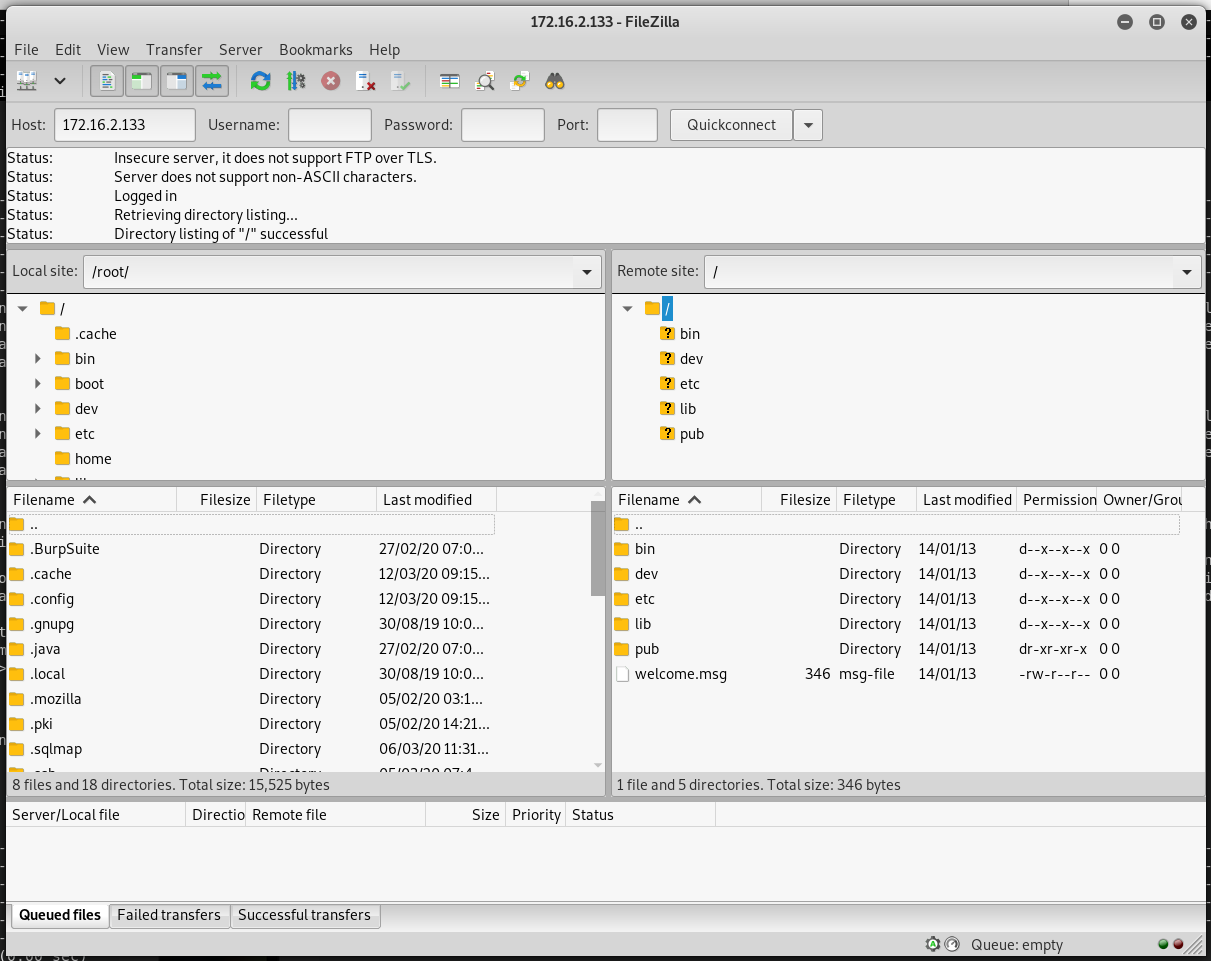
\includegraphics[scale=0.4]{img/ftp1.png}
	\caption{FTP access using anonymous user}
\end{figure}
\begin{figure}[!htb]
	\centering
	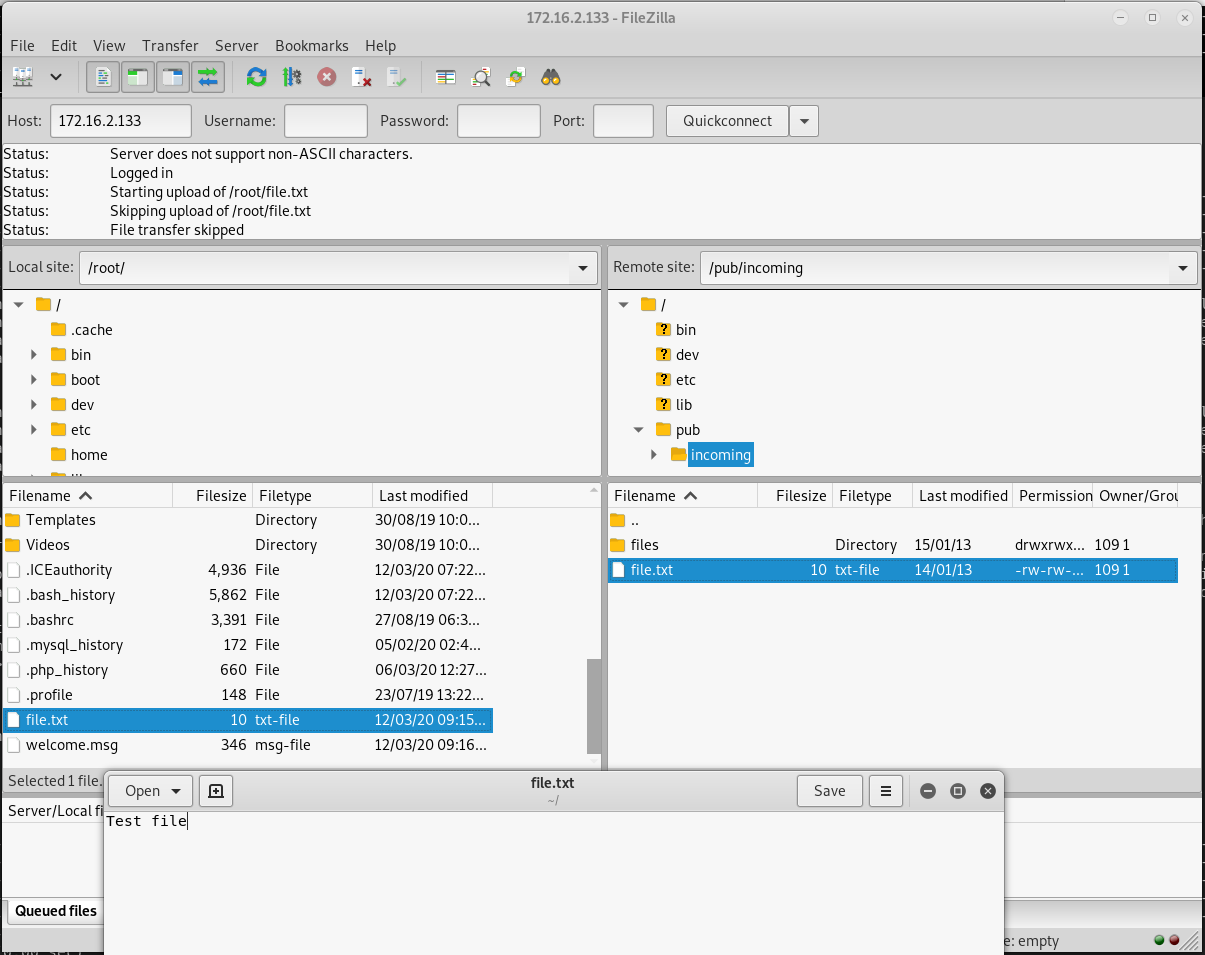
\includegraphics[scale=0.4]{img/ftp2.png}
	\caption{Retrieving files from the server}
\end{figure}
\pagebreak

\subsection{SSH Bruteforce}
\subsubsection{Security Implications / Risk Level}
SSH, or Secure Shell, is a service that allows users to gain command line access to a remote machine. While this is a useful tool for managing machines without having physical access, it also gives threat actors a lucrative target.\\
One common method used by threat actors to gain access to SSH is an SSH bruteforce. Similar to the RDP bruteforce used on SRV1, this tries a lot of passwords repeatedly, hoping for one to be correct.\\
While this exploit does have serious ramifications if executed correctly, the slow speed of SSH bruteforcing combined with the ease of use securing SSH sets the risk to \textbf{medium}.
\subsubsection{Cause of Vulnerability}
This vulnerability is caused by a few factors:
\begin{itemize}
	\item Lack of IP blocking - a common measure is to block IPs if they repeatedly try to access SSH incorrectly, forcing the attacker to use a botnet instead.
	\item Lack of strong passwords - the passwords found for the accounts were both weak, appearing within the rockyou.txt wordlist. Choosing stronger passwords makes it much more difficult for the threat actor to effectively bruteforce.
	\item Using the default SSH port - this is more of an issue with automated bots, but using the default SSH port (22) advertises the use of the port, giving easier access to the entry point for threat actors.
\end{itemize}
\subsubsection{Steps to Reproduce}
\begin{itemize}
	\item The usernames gained from viewing /etc/passwd through path traversal were collated in to a wordlist.
	\item The tool hydra was again used to brute force, using the above wordlist for the usernames and rockyou.txt for passwords. The command used was:
	\begin{verbatim}
	hydra -L usernames.txt -P rockyou.txt 172.16.2.133 -t 4 ssh
	\end{verbatim}
	\item After allowing the bruteforce to run for a few hours, it produced two sets of credentials - 'hr\_kx:password' (Fig. 3.27), and 'gshear:swordfish' (Fig. 3.28).
	\item These credentials were then tested for use with SSH. The hr\_kx user had no shell privileges, so could not be used to execute commands. The gshear user did have privileges, and was used to gain access to the system.
\end{itemize}
\begin{figure}[!htb]
	\centering
	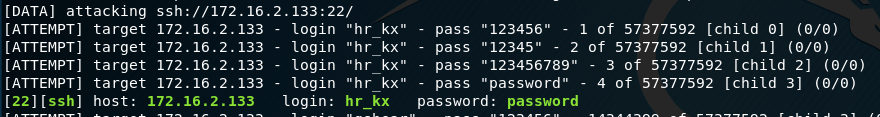
\includegraphics[scale=0.5]{img/133ssh1.png}
	\caption{kr\_kx cracked}
\end{figure}
\begin{figure}[!htb]
	\centering
	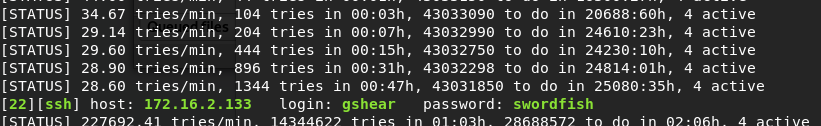
\includegraphics[scale=0.6]{img/133ssh2.png}
	\caption{gshear cracked}
\end{figure}
\pagebreak

\subsection{Improper Access Controls}
\subsubsection{Security Implications / Risk Level}
Access controls are used to limit which users are allowed to access certain functionalities on a system. For example, only users with root access can edit important system files on Linux machines.\\
In this case, read permissions were inadvertently left accessible to non-privileged users in the /var/www directory. This allowed for sensitive mysql data to be accessed in the conn.php script, which lead to more vulnerabilities being created.\\
As the potential risks of this vulnerability can be so broad, and said risks are easily executable once access has been gained to the system, this vulnerability is assessed to be of \textbf{high} risk.
\subsubsection{Cause of Vulnerability}
This vulnerability is caused by a lack of consideration when configuring user access on files and services. This is a common mistake made by sysadmins when setting up a server, as making considerations for which levels of privilege each user should have is a time-consuming task.
\subsubsection{Steps to Reproduce}
\begin{itemize}
	\item The first step was to navigate to the /var/www folder, where Apache web files are stored. This is a common site for improper access control - non-privileged users are often able to edit the files here, or view them and recover important information.
	\item In the 'graphite' folder containing all site data, there was a file named 'conn.php'. A file like this is usually for handling the connection between the server and the database, so it was worth checking.\\
	Inside, the details for the MySQL user 'auctuser' were stored in plaintext (Fig. 3.29).
	\item With these details, it was possible to log in to the MySQL server using the command
	\begin{verbatim}
		mysql -u auctuser -p
	\end{verbatim}
	Followed by the password, 'figel'. Once in the database, it was possible to not only read data, but to insert data too.
	\item One way this could be exploited is by achieving XSS on the homepage. Due to the way auctions are stored, without stripping HTML tags, it was possible to craft a special INSERT INTO query to insert XSS into the description field of the generated auction (Fig. 3.30).
	\item With this done, the homepage could be refreshed to display an alert(1) box, showing the vulnerability working as intended (Fig. 3.31). This could be used as a method of persistence, continually stealing session IDs or logging their keystrokes using Javascript.
\end{itemize}
\begin{figure}[!htb]
	\centering
	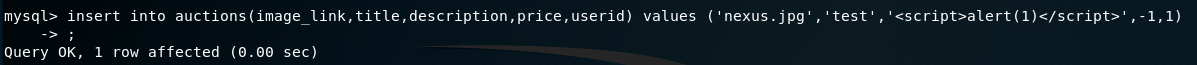
\includegraphics[scale=0.6]{img/xss1.png}
	\caption{Viewing MySQL details}
\end{figure}
\begin{figure}[!htb]
	\centering
	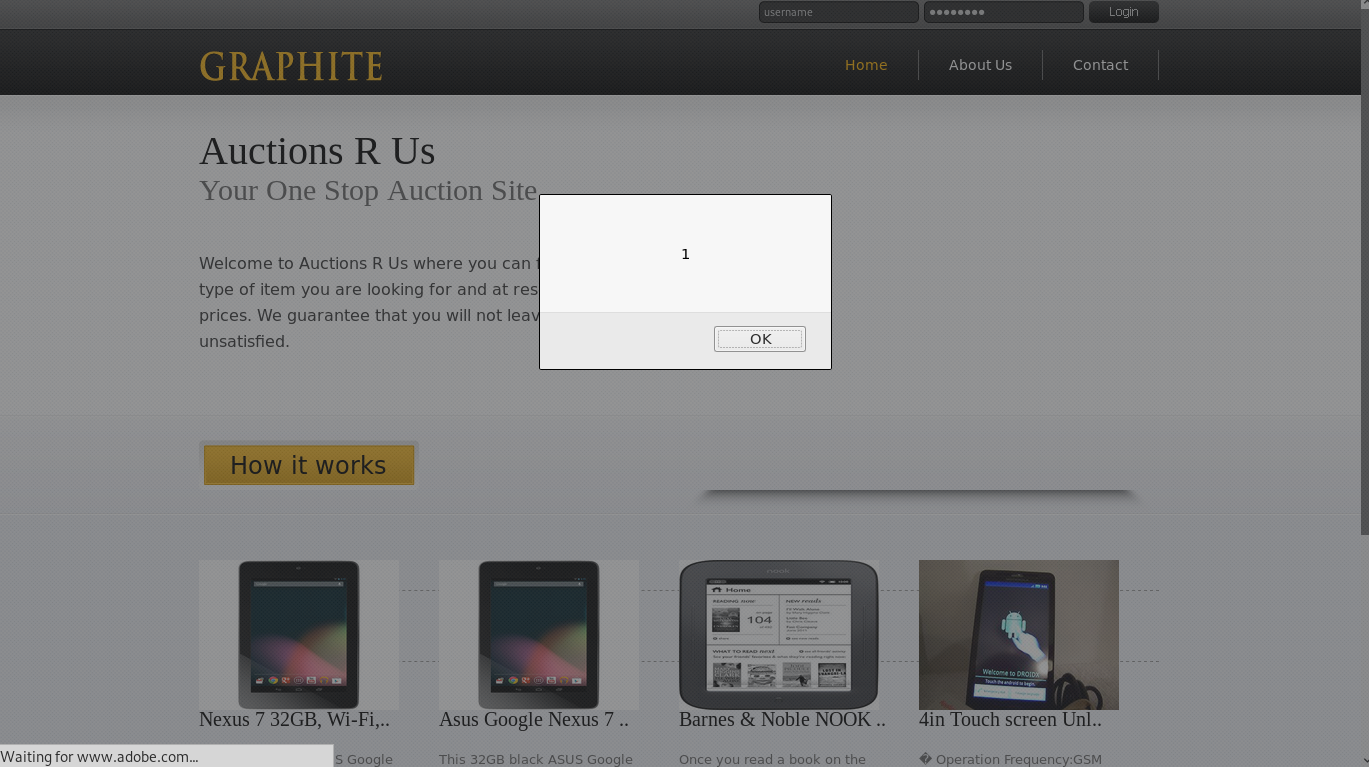
\includegraphics[scale=0.4]{img/xss2.png}
	\caption{Injecting XSS through the DB}
\end{figure}
\begin{figure}[!htb]
	\centering
	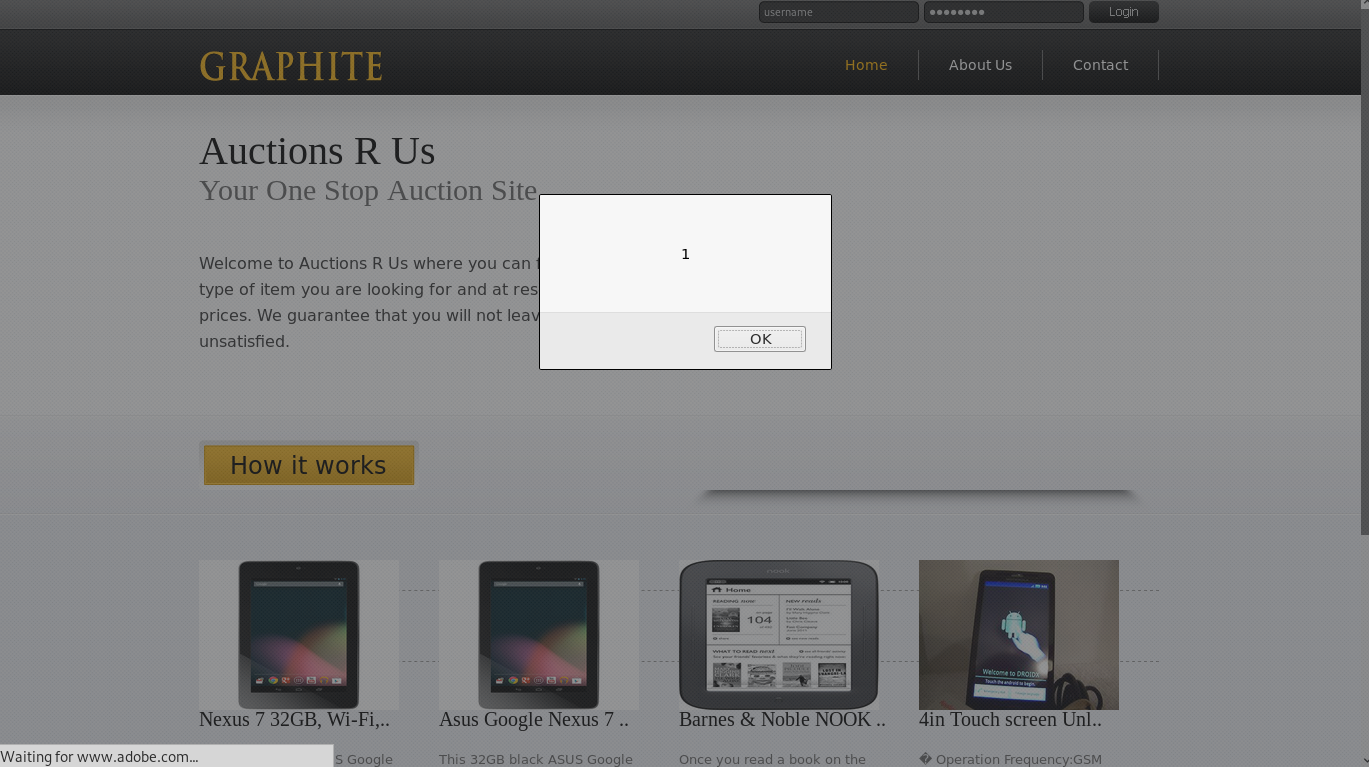
\includegraphics[scale=0.3]{img/xss3.png}
	\caption{Demonstrating XSS}
\end{figure}
\pagebreak

\section{SRV2 - Linux Server}
\subsection{Username Enumeration}
\subsubsection{Security Implications / Risk Level}
Username enumeration allows threat actors to identify some or all of the users present on a  remote machine. While this may not seem dangerous on its own, when combined with other attacks (such as SSH or RDP bruteforce) it can enable further access than would otherwise be possible.\\
In this case, using username enumeration allowed for an SSH bruteforce attack to occur, eventually leading to SSH access being gained on the machine.\\
Due to the low potential payload of the vulnerability and relative difficulty to access, this vulnerability is assessed as \textbf{low} risk.
\subsubsection{Cause of Vulnerability}
There are a variety of ways usernames can be leaked by some services - in this case, the usernames were gained by using enum4linux to enumerate SIDs with null SMB credentials, yielding the username. Another common exploit is to use a malformed packet vulnerability in SSH along with a wordlist to bruteforce specific usernames \cite{userenum}.
\subsubsection{Steps to Reproduce}
\begin{itemize}
	\item The username enumeration process was done with the tool enum4linux, included with Kali. The command used was:
	\begin{verbatim}
	enum4linux 172.16.2.140 -a
	\end{verbatim}
	This performs all common enumeration techniques on the target machine.
	\item When completed, the program returned the results of enumerating SIDs using a null SMB credential attack. This yielded the username 'ktuser', with SID S-1-22-1-1000(Fig. 3.32).
\end{itemize}
\begin{figure}[!htb]
	\centering
	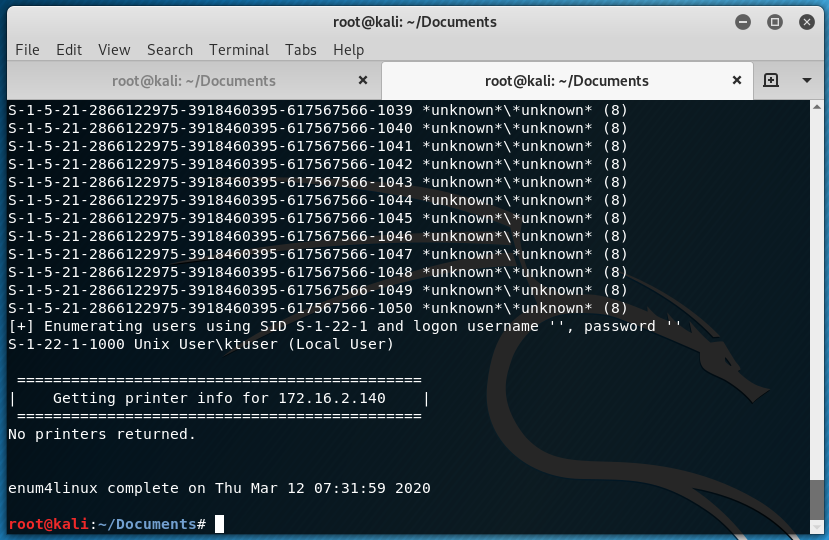
\includegraphics[scale=0.6]{img/userenum1.png}
	\caption{Enumerating users}
\end{figure}

\subsection{SSH Bruteforce}
\subsubsection{Security Implications / Risk Level}
This SSH bruteforce is functionally identical to the one performed on the Ubuntu machine, and therefore has the same risk rating of \textbf{medium}.
\subsubsection{Cause of Vulnerability}
Identical to Ubuntu SSH - combination of lack of IP blocking, lack of strong passwords, and using the default SSH port.
\subsubsection{Steps to Reproduce}
\begin{itemize}
	\item Again, Hydra was used for this SSH bruteforce. Instead of just one bruteforce running, multiple were set up concurrently - each with different rules. These were:
	\begin{itemize}
		\item A standard bruteforce using rockyou.txt
		\item A bruteforce using the top 10 million passwords list
		\item A bruteforce using the xato net passwords list
		\item A bruteforce using an exhaustive lowercase search
		\item A bruteforce using an exhaustive lowercase/uppercase search
		\item A bruteforce using an exhaustive lowercase/uppercase/numbers/symbols search
	\end{itemize}
	This was done to maximise the chances that at least one would succeed.
	\item After allowing the bruteforces to run, the exhaustive lowercase search came up with a result - 'ktuser:aaa' (Fig. 3.33). This showed that the multiple bruteforce attack was effective, as the string 'aaa' does not appear in rockyou until a few thousand in, while it only took less than 300 attempts with an exhaustive search.
	\item The credentials could then be used to SSH in to the machine successfully, gaining a shell.
\end{itemize}
\begin{figure}[!htb]
	\centering
	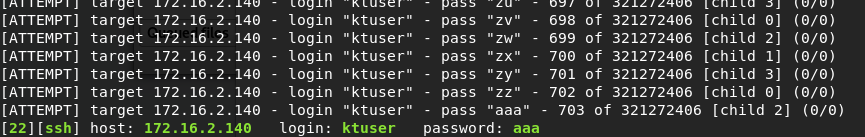
\includegraphics[scale=0.6]{img/140ssh1.png}
	\caption{Enumerating users}
\end{figure}





\chapter{Recommendations}
\section{Auction Site}
\subsection{Path Traversal}
\subsection{SQL Injection}
\subsection{Weak Authentication}

\section{SRV1 - Windows Server}
\subsection{RDP bruteforce}
	change or close port
\subsection{Insecure privileges}
In a secure system, principles such as the 'rule of least privilege' should be used.
\subsection{Weak passwords}

\section{Ubuntu Client}
\subsection{SSH bruteforce}

\section{SRV2 - Linux Server}



\chapter{Conclusion}

\chapter{Appendices}
\section{Appendix A: Python bruteforce script}
\begin{figure}[!htb]
	\centering
	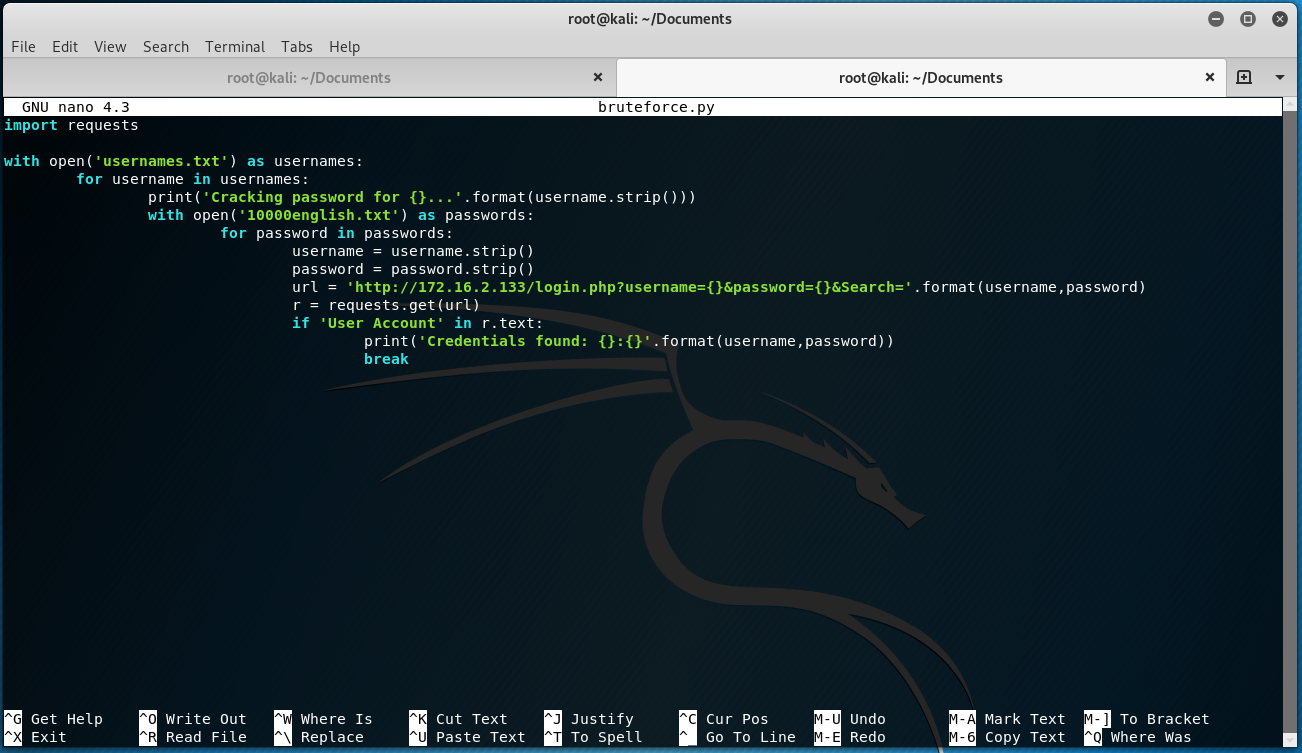
\includegraphics[scale=0.4]{img/bruteforcescript.png}
	\caption{Login form bruteforce script}
\end{figure}
\section{Appendix B: Session enumeration script}
\begin{figure}[!htb]
	\centering
	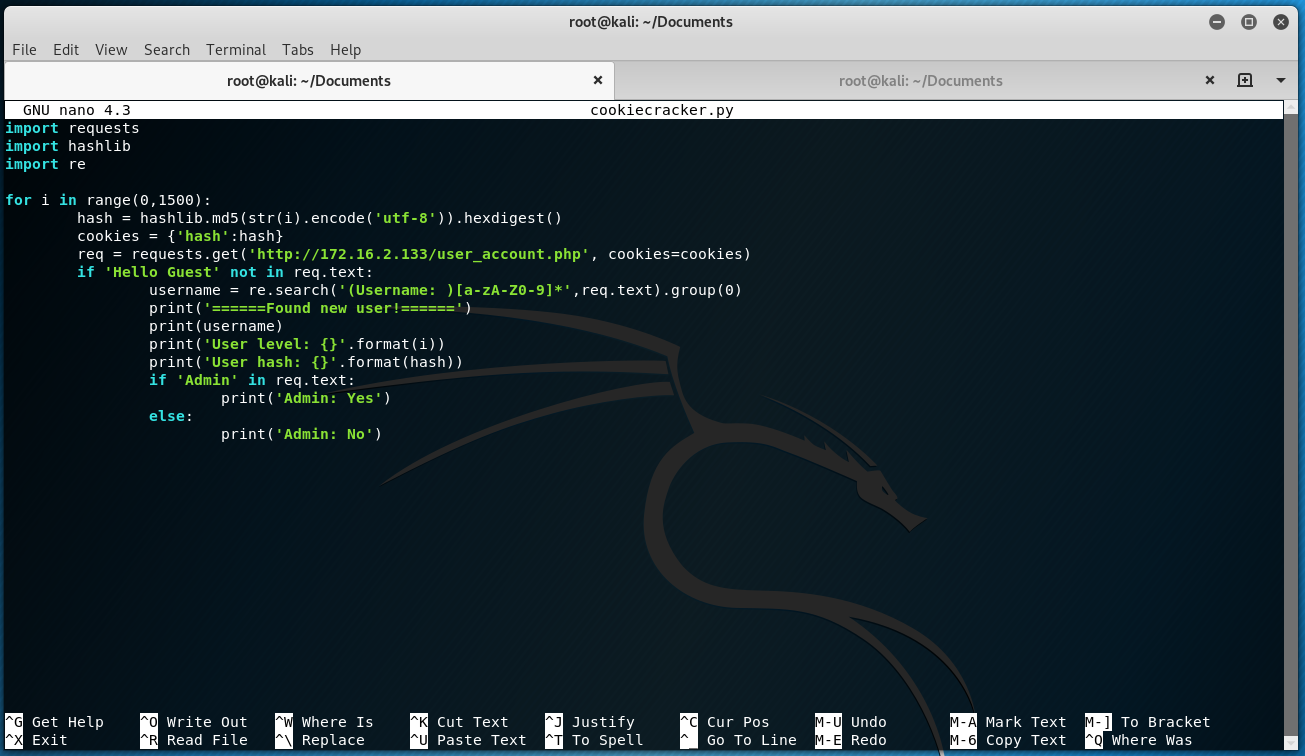
\includegraphics[scale=0.4]{img/cookiescript.png}
	\caption{Enumerating the session cookies}
\end{figure}

\bibliography{pentest}

\end{document}